\documentclass[paper=a4, fontsize=11pt]{scrartcl}
\usepackage{enumerate}
\usepackage{amsmath}
\usepackage{amssymb}
\usepackage{tikz}
\newcommand{\parens}[1]{ \left( #1 \right) }
\begin{document}
\noindent Willy Xiao and Kevin Eskici \\ STAT 221 \\Pset 5\\ Nov 18, 2014
\begin{enumerate}[\text{question }1.]
  \item
    \begin{enumerate}[1]
      \item Figure 2 Replica. See $keskici\_wxiao\_1router.R$ for code \\
      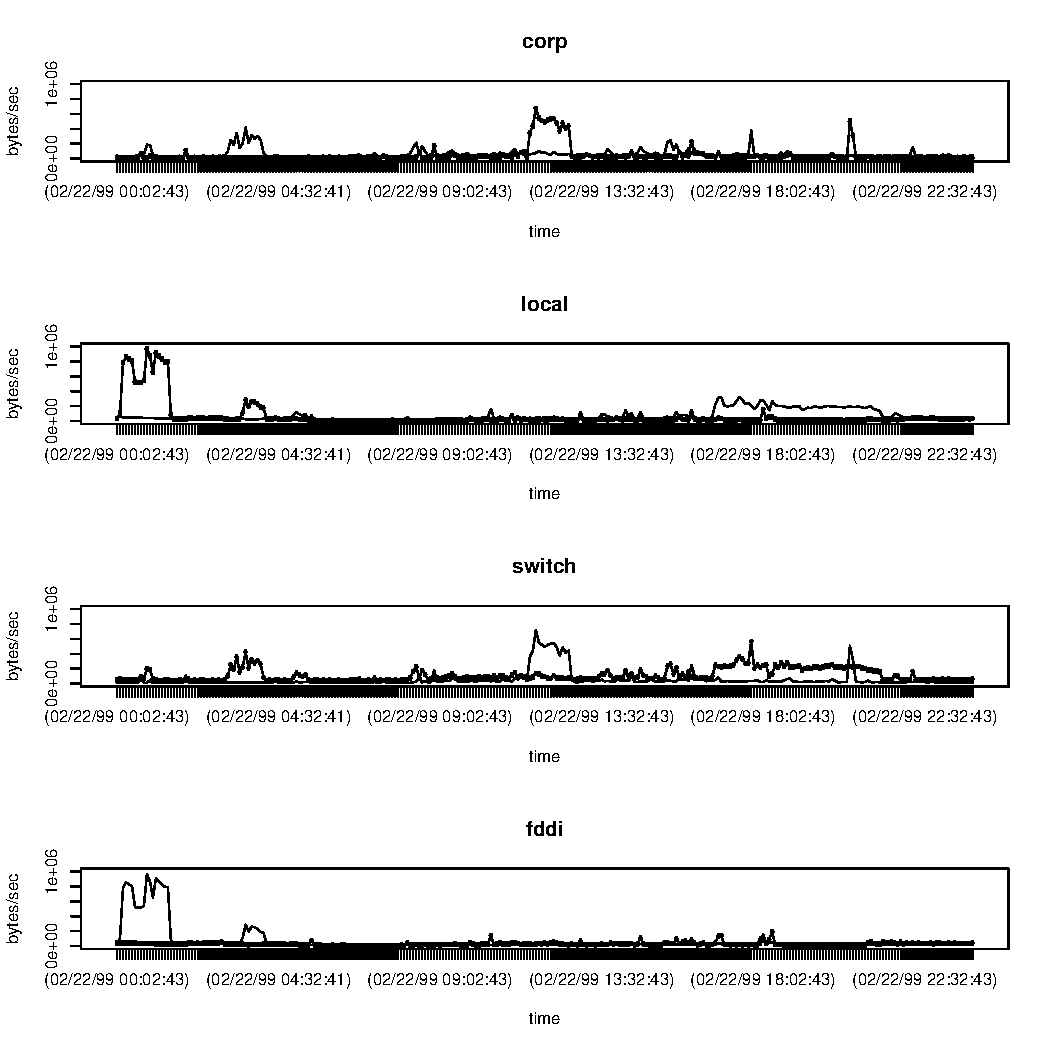
\includegraphics[scale=.8]{keskici_wxiao_fig2.pdf}
      \newpage
      \item Figure 4 replica for $1router\_allcount.dat$ \\
      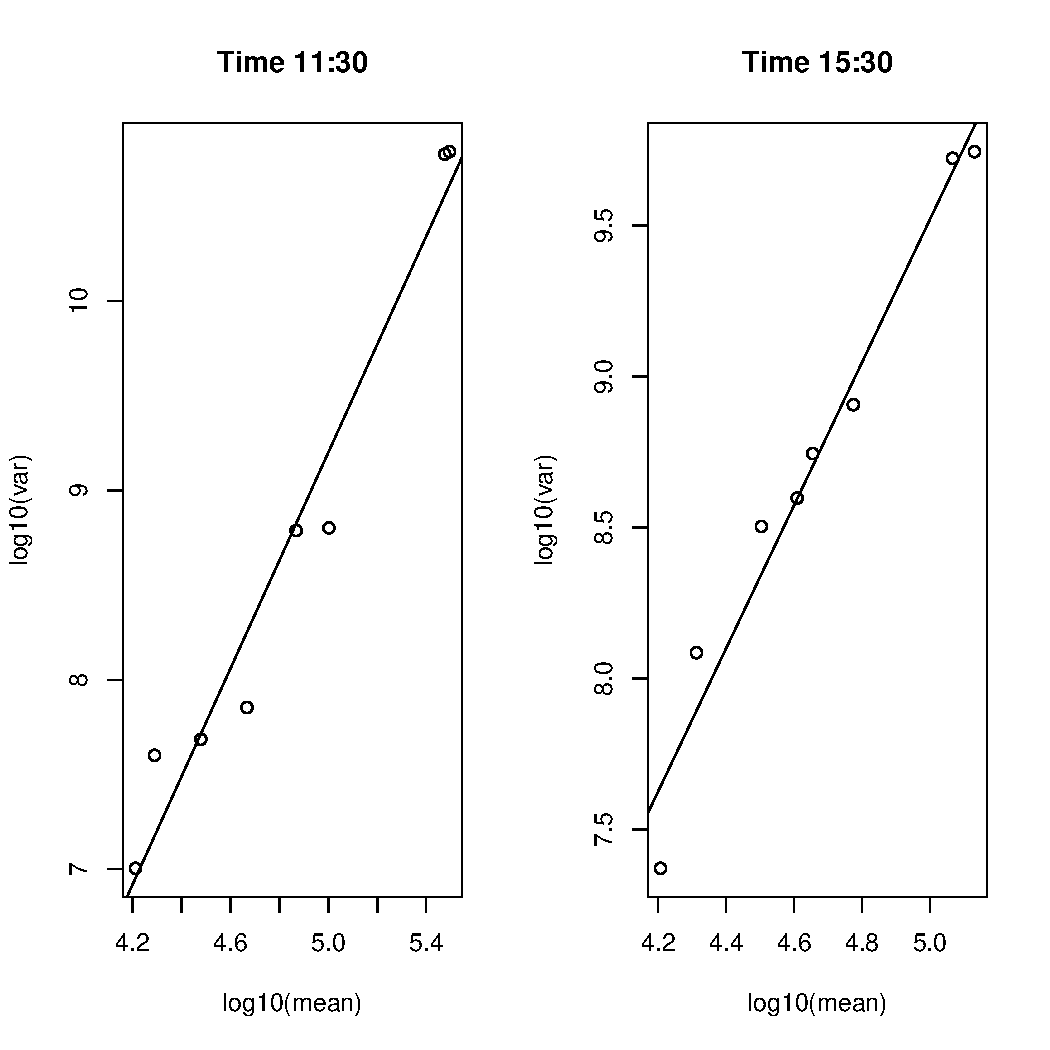
\includegraphics[scale=.8]{keskici_wxiao_fig4_1router.pdf}\\
      \newpage
      Figure 4 Replica for $2router\_linkcount.dat$ \\
      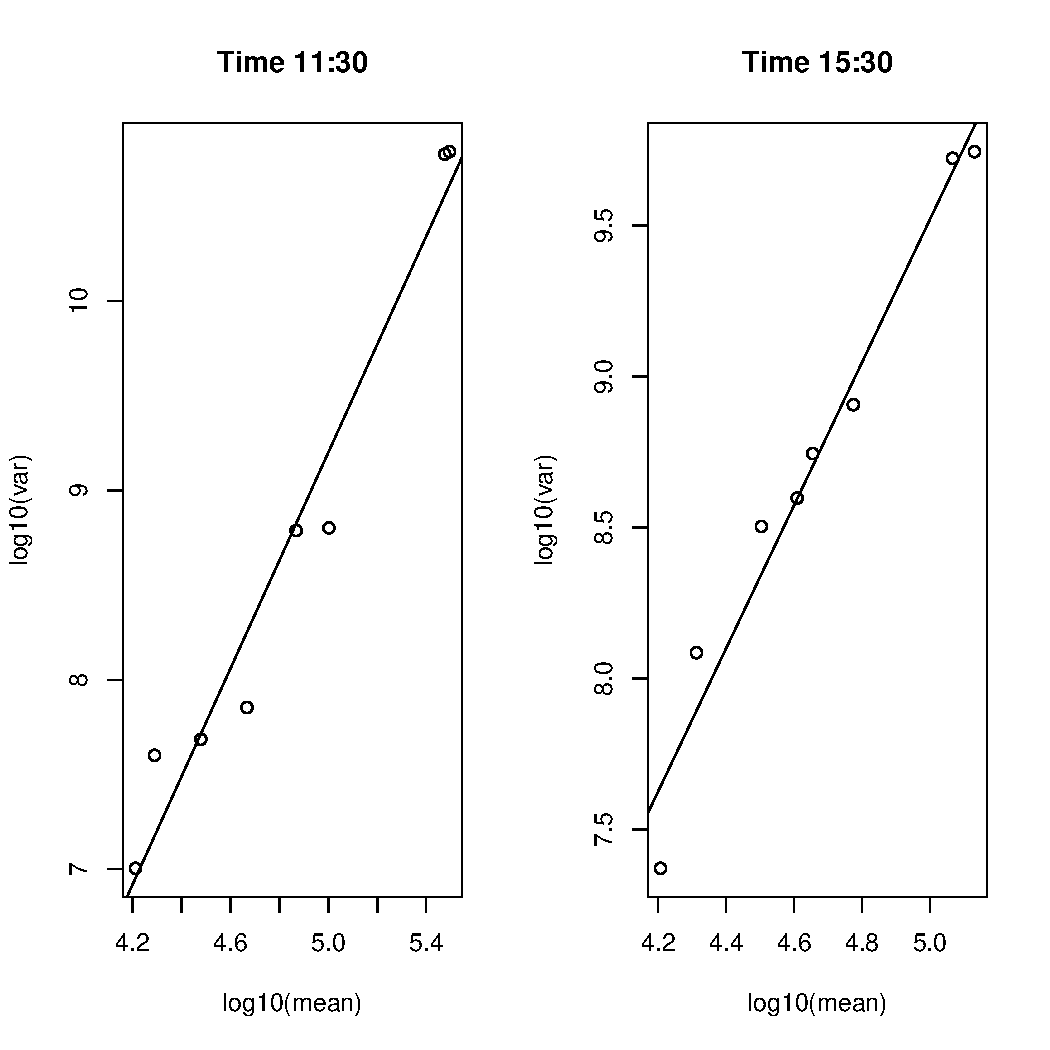
\includegraphics[scale=.8]{keskici_wxiao_fig4_1router.pdf}

      \item
        \begin{enumerate}[a.]
          \item
          \begin{align*}
            Q(\theta, \theta^k) &= E(l(\theta|X)|Y, \theta^k) \\
            &= E(-T/2\log{|\Sigma|} - 1/2\sum{(x_t-\lambda)'\Sigma^{-1}(x_t - \lambda)}) \\
            &= -T/2\log{|\Sigma|} - 1/2*\sum{E(m_t^k - \lambda)'\Sigma^{-1}(m_t^k - \lambda)) + tr(\Sigma^{-1}R^{k})} \\
            &= -T/2(\log{|\Sigma|} + tr(\Sigma^{-1}R^k)) - 1/2\sum_{t=1}^{T}{(m\_t^{(k)} - \lambda)'\Sigma^{-1}(m_t^{(k)} - \lambda)}
          \end{align*}
          \item Pseudocode:
            \begin{enumerate}[I.]
              \item Set $x = \vec{0}$, $v = \vec{0}$
              \item For each $y_t$ do \\
                \indent $v := Concat(v, y_{t,1})$ \\
                \indent $x := x + y_t$
              \item Set $\lambda_0 = \overrightarrow{1'(x/w)}$, $\phi_0 = var(v)/mean(v)$.
              \item Initialize $\theta^{(0)} = \theta_0 = (\lambda_0, \phi_0)$.
              \item Until $\theta^{(k+1)} = \theta^{(k)}$ do \\
                \begin{tabbing}
                  \hspace{1cm} $Q := (\theta, \theta^{(k)})$ do: \\
                  \hspace{2cm} $\Sigma := \phi*diag(\lambda_1^c, \ldots, \lambda_I^c)$. \\
                  \hspace{2cm} $\Sigma^{(k)} := \phi^{(k)}*diag((\lambda_1^{(k)})^c, \ldots, (\lambda_I^{(k)})^c)$ \\
                  \hspace{2cm} $R^{(k)} := \Sigma^{(k)} - \Sigma^{(k)}A'solve(A\Sigma^{(k)}A')A\Sigma^{(k)}$ \\
                  \hspace{2cm} $S := $ sum for each $t$: \\
                  \hspace{3cm} $m := \lambda^{(k)} + \Sigma^{(k)}A'solve(A\Sigma^{(k)}A')(y_t - A\lambda^{(k)})$ \\
                  \hspace{3cm} return $(m - \lambda)'\Sigma(m - \lambda)$. \\
                  \hspace{2cm} return $-\frac{T}{2}\log{|\Sigma|} + tr(solve(\Sigma)R^{(k)}) - (1/2)S$. \\
                  \hspace{1cm} $\theta^{k} := \theta^{(k+1)}$ \\
                  \hspace{1cm} $\theta^{(k+1)} := optim(Q)$
                \end{tabbing}
            \end{enumerate}
        \end{enumerate}
        \newpage
      \item For the local iid model, instead of initializing with all $y_t$ we initialize with $y_t \in [y_{t - w/2}, y_{t+w/2}]$ and we also sum only over those $t \in [t - w/2, t + w/2]$. \\ \includegraphics[scale=.8]{keskici_wxiao_fig5.pdf}
      \item The refined model is, after choosing V just \\
      \begin{align*}
        p(\eta_t|\widetilde{Y_t}) &= p(\eta_t|\widetilde{Y}_{t-1}, Y_t) \propto p(\eta_t|\widetilde{Y}_{t-1})p(Y_t|\eta_t) \\
        p(\eta_t|\widetilde{Y}_{t-1}) &\sim N(\hat{\eta}_{t-1}, \hat{\Sigma}_{t-1})
      \end{align*}
      Where
      \begin{align*}
        \hat{\Sigma}_{t-1} &= g''(\eta_t)^{-1} = -\hat{\Sigma}^{-1}_{t|t-1} + \partial^2{\log{p}}/\partial{\eta_t}^2 \\
        & \text{ and the second derivative is defined on page 1067. } \\
        & \text { We just used the hessian function. }
      \end{align*}
      \newpage
      \item See R code for fitting\\
      \includegraphics[scale=.8]{keskici_wxiao_fig6_1router.pdf}
      \newpage
      \item There is no 1.7 in the pset...
      \item In general the Tebaldi-West method should be pretty similar to the CaoYu method in producing the final outputs. In many ways, Tebaldi-West will be even better because it doesn't approximate the poisson with a normal model that CaoYu does. The issue; however, is that the Tebladi-West algorithm will take a long time to run (even for the case of the Markov-Gibbs algorithm). In a sense you can think that Tebaldi-West throws a ton of darts at a board to find the maximium likelihood for $x_t$; while CaoYu is starting at the edge of the boarding and walking closer and closer to the best $x_t$ (ie the EM is moving towards the better values).
      \item See R code for fitting.Note: Since we didn't use SLURM (which Panos said was fine-we ran our code on a separate external server) the code for this part takes awhile to run (on the order of several hours). In case you don't want to run it for that long, we've included the RData files \\
      \newpage
      Eqivalent of Figure 6 for $2router\_linkcount.dat$\\
      \includegraphics[scale=.4]{keskici_wxiao_fig6_2router.pdf}\\
      \newpage
      Equivalent of Figure 5 for $2router\_linkcount.dat$-not oficially asked for but we were asked to fit
      the locally iid model so seemed natural to include it\\
      \includegraphics[scale=.4]{keskici_wxiao_fig5_2router.pdf}

    \end{enumerate}
\end{enumerate}
\end{document}
